\section{Algorithm Output}
My implementation of the linear-Gaussian binary latent feature model with the IBP prior generates the results in images and traceplots. The simulated dataset contains four latent features (see Figure~\ref{fig:images}), and my code reveals all of them in Figure~\ref{fig:imageresults}. Note that my Gibbs sampler is sensitive to the random seed settings, and using another random seed in the code initialization reveals five (instead of four) latent features in Figure~\ref{fig:imageresultsK5}, three of which are the linear combinations of two latent features.\\ 

The traceplots in Figure~\ref{fig:plotresults} show my Gibbs sampler is converging: $K_+$ fluctuates between 5 and 8; the IBP parameter $\alpha$ is within (0.2,3.0); $\sigma_X$ converges to the true value 0.5; $\sigma_A$ oscillates around 0.4. A total of 1000 Gibbs sampling iterations were performed, but the values started to converge at the 100th iteration. Figure~\ref{fig:hist} shows the histogram of sampled $K_+$ values and the number of features for each object in the final iteration of $\mathbf{Z}$. The correct $K_+ = 4$ is not the sampled value with the highest probability, but the majority of objects only contain at most 4 features, so I conclude that $K_+ > 5$ in the middle of iterations are due to extreme values. \\

% Histograms, new images comparison :)
Moreover, the latent feature model is able to "reverse" the noisy images to the linear combination of latent features. Figure~\ref{fig:reverse} is an example of the first four images in the simulated dataset: The top row contains the "reversed" images, and the latent features in each one can be clearly seen. The bottom row represents the original images, in which the latent features are obscured by the random noise. The binary strings on top of all images indicate which bases are present in which image; for example, the string "1100" represents an image as a linear combination of the first and second bases, without the third and fourth ones.

\begin{figure}[!ht]
\centering
    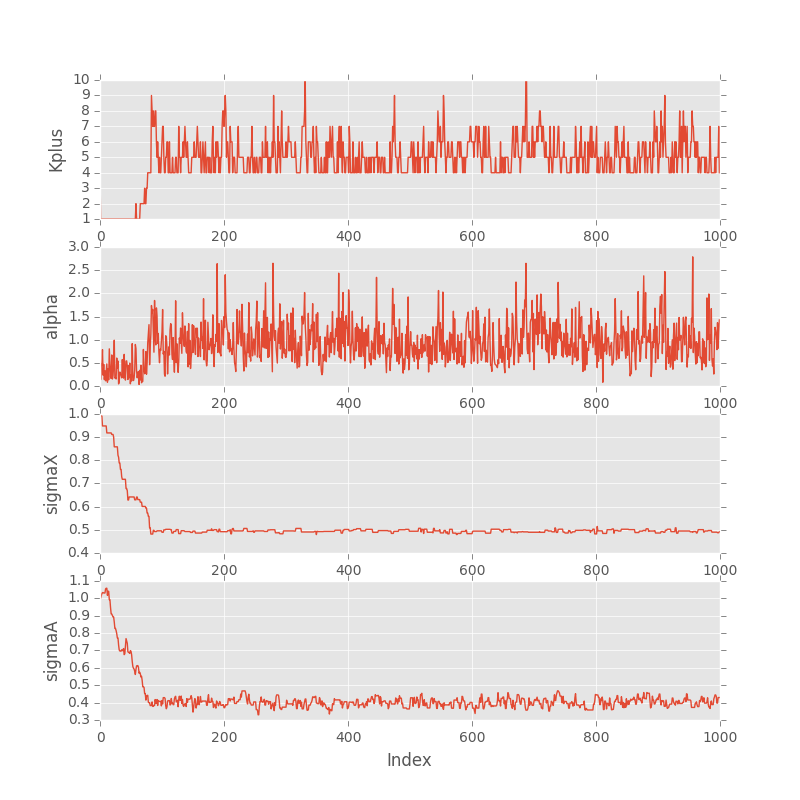
\includegraphics[width=0.65\linewidth]{Version1_Naive_Code/IBP_plot_results.png}
    \vspace{-20pt}
    \caption{The traceplots for $K_+, \alpha, \sigma_X, \sigma_A$}
    \label{fig:plotresults}
\end{figure}

\begin{figure}[!ht]
\centering
    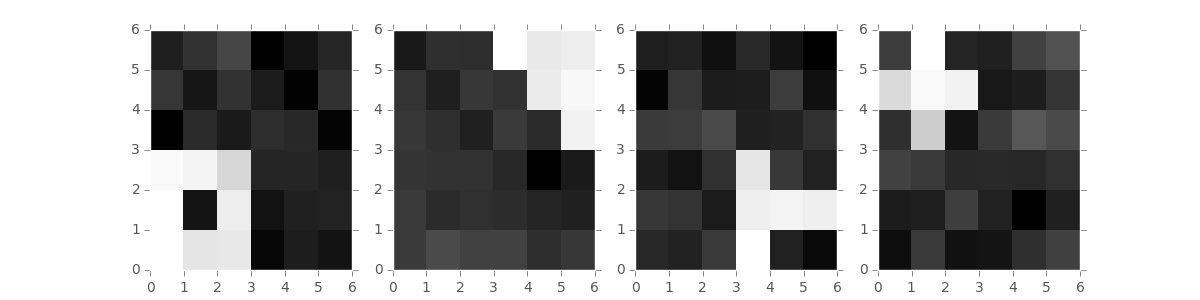
\includegraphics[width=\linewidth]{Version1_Naive_Code/IBP_image_results.png}
    \caption{Simulated dataset: My results}
    \label{fig:imageresults}
\end{figure}

\begin{figure}[!ht]
\centering
    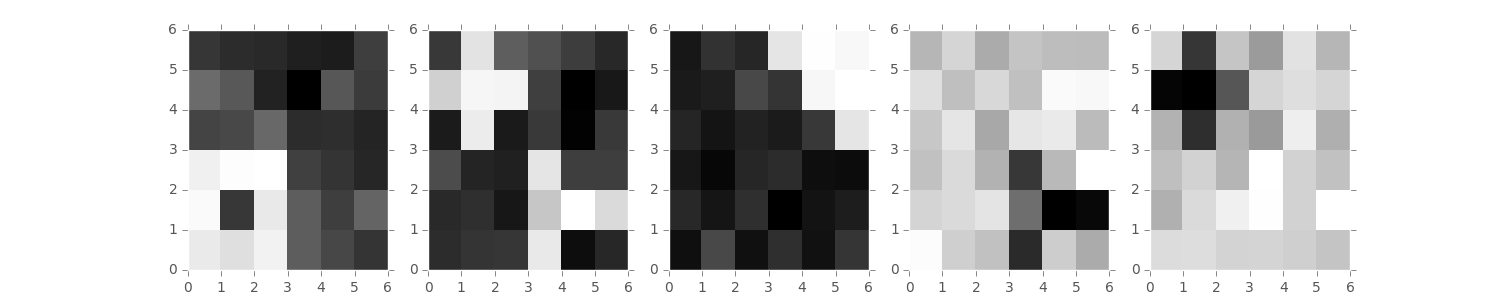
\includegraphics[width=\linewidth]{Version0_Wrong/IBP_image_results_K5.png}
    \caption{Simulated dataset: My results with another random seed}
    \label{fig:imageresultsK5}
\end{figure}

\begin{figure}[!ht]
\centering
    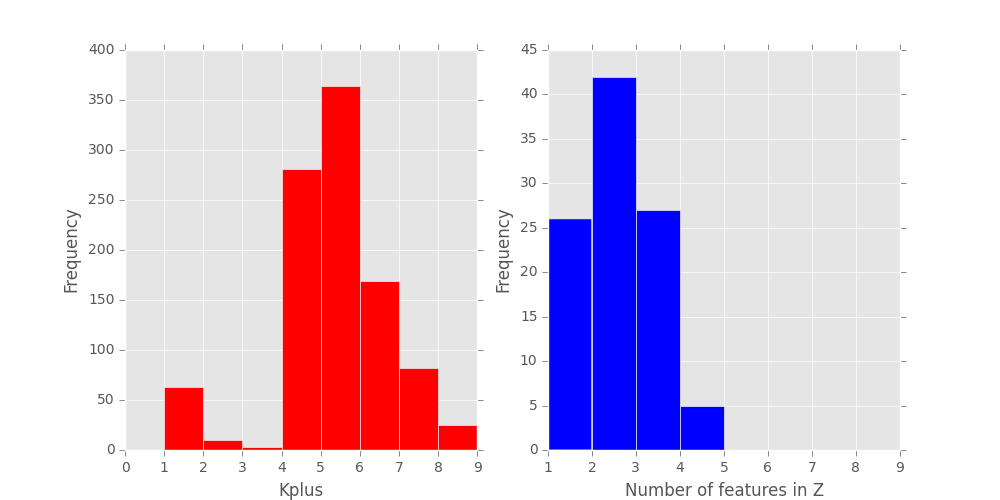
\includegraphics[width=0.8\linewidth]{Reverse/IBP_Histograms.png}
    \caption{Histograms of $K_+$ (left) and the number of features in $\mathbf{Z}$ (right)}
    \label{fig:hist}
\end{figure}

\begin{figure}[!ht]
\centering
    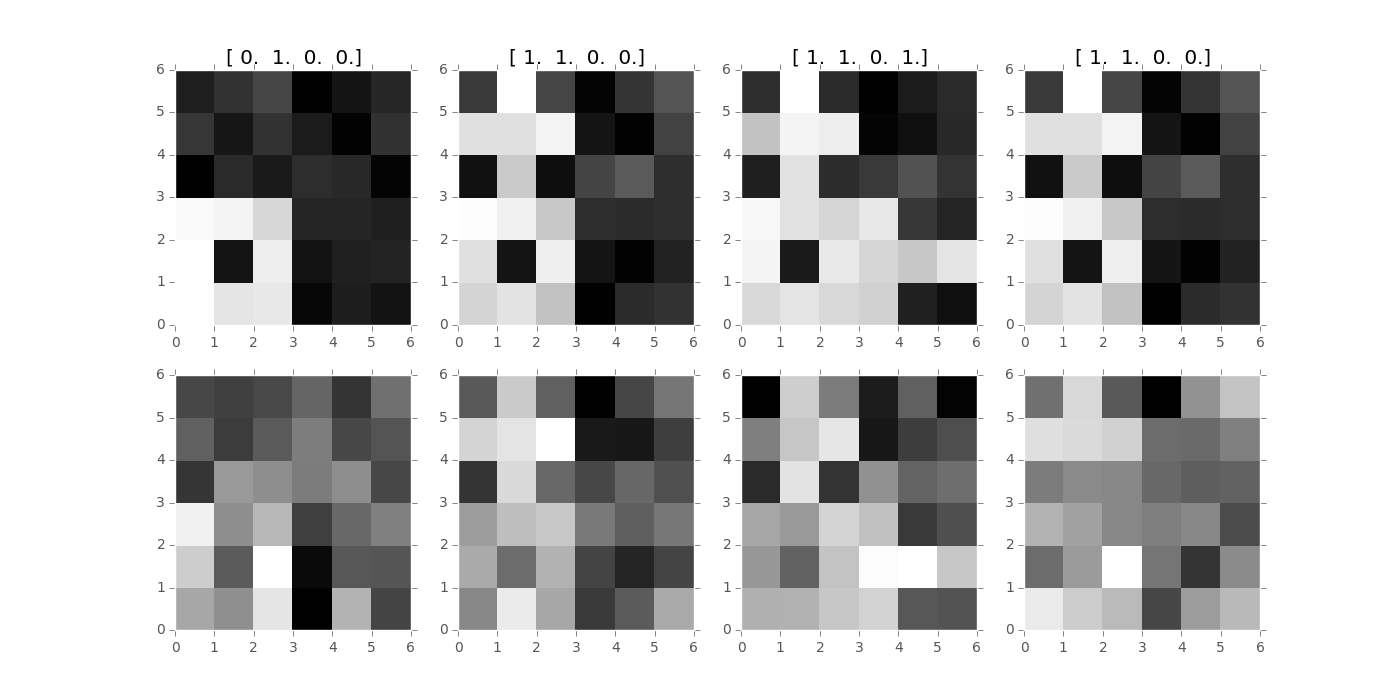
\includegraphics[width=\linewidth]{Reverse/IBP_Reverse_Images.png}
    \caption{The latent features (top) corresponding to the simulated images (bottom)\\
    The binary strings on top of all images indicate which bases are present in which image.\\
    From left to right: 0100, 1100, 1101, 1100}
    \label{fig:reverse}
\end{figure}
